\documentclass[10pts]{article}

%% Language and font encodings
\usepackage[english]{babel}
\usepackage[utf8x]{inputenc}
\usepackage[T1]{fontenc}
\usepackage{float}
\usepackage{listings}
\usepackage{nicefrac}
%% Sets page size and margins
\usepackage[letterpaper,top=3cm,bottom=2cm,left=3cm,right=3cm,marginparwidth=1.75cm]{geometry}

%% Useful packages
\usepackage{amsmath}
\usepackage{amsthm}
\usepackage{graphicx}
\usepackage{subcaption}
\usepackage{color}
\usepackage{xcolor}
\usepackage[colorlinks,allcolors=blue]{hyperref}
\usepackage{cleveref}
\usepackage{booktabs}
\usepackage{multirow}
\usepackage{paralist}
\usepackage{cite}
%\definecolor{codegreen}{rgb}{0,0.6,0}
%\definecolor{codegray}{rgb}{0.5,0.5,0.5}
%\definecolor{codepurple}{rgb}{0.58,0,0.82}
%\definecolor{backcolour}{rgb}{0.95,0.95,0.92}

\newif\ifdraft
\drafttrue
\ifdraft
\definecolor{ocolor}{rgb}{1,0,0.4}
\newcommand{\jwave}[1]{ {\reduwave{#1}}}
\newcommand{\jhanote}[1]{ {\textcolor{red} { ***shantenu: #1 }}}
\newcommand{\mtnote}[1]{ {\textcolor{cyan} { ***matteo: #1 }}}
\definecolor{orange}{rgb}{1,.5,0}
\definecolor{dandelion}{cmyk}{0,0.29,0.84,0}
\newcommand{\gpnote}[1]{{\textcolor{green} {***giannis: #1}}}
\newcommand{\note}[1]{ {\textcolor{magenta} { ***Note: #1 }}}
\else
\newcommand{\jwave}[1]{}
\newcommand{\jhanote}[1]{}
\newcommand{\mtnote}[1]{}
\newcommand{\gpnote}[1]{}
\newcommand{\note}[1]{}
\fi

\theoremstyle{definition}
\newtheorem{defn}{Definition}[section]

\lstdefinestyle{mystyle}{
    backgroundcolor=\color{backcolour},   
    commentstyle=\color{codegreen},
    keywordstyle=\color{magenta},
    numberstyle=\tiny\color{codegray},
    stringstyle=\color{codepurple},
    basicstyle=\footnotesize,
    breakatwhitespace=false,         
    breaklines=true,                 
    captionpos=b,                    
    keepspaces=true,                 
    numbers=left,                    
    numbersep=5pt,                  
    showspaces=false,                
    showstringspaces=false,
    showtabs=false,                  
    tabsize=2
}
 
\lstset{style=mystyle}

\title{Autonomic workload manager for executing scientific workflows on High Performance Computing resources}
\author{Ioannis Paraskevakos \\	Electrical and Computer Engineering \\
        Rutgers, The State University of New Jersey}

\begin{document}
\maketitle

\abstract{Many scientific application workflows are becoming larger and need to be executed multiple times with different parameters, generating a scientific computational campaign. Domains such as molecular dynamics, biological, and environmental sciences, define workflows and pipelines that are executed $O(1k)$ to $O(10k)$ times. In addition, based on results obtained during runtime the application computational requirements may change. Managing computational resources to reduce time to completion, maximize utilization, and maximize scientific insight, is becoming necessary. In this proposal, we present research done to understand:
    \begin{inparaenum}[(i)]
        \item scientific application time to completion characterization,
        \item scalability behavior of scientific workflows based on programming models.
       \end{inparaenum}
We summarize preliminary results from our research for modeling scientific workflows in terms of time to completion, and propose an autonomic workload manager to manage workflow execution on High Performance resources. We include a work plan to investigate, formulate and implement the proposed workload manager and evaluate foreseen challenges and risks.}


\section{Introduction}
\label{ch:intro}
This is the introduction of my dissertation. This document will try to show all the details of my work over the last six years.

\begin{figure}
    \centering
    \includegraphics{}
    \caption{Caption}
    \label{fig:my_label}
\end{figure}

\section{Working Definitions}
Terms such as ``workflow'', ``workload'', ``autonomic computing'' are usually overloaded in literature  and defined differently across domains. As a result, we define the terminology used in this proposal:
\begin{itemize}
    \item \textbf{Autonomic Computing}: Based on the definition by IBM~\cite{ibm2005autonomic}, it is a computing environment with the ability to manage itself and dynamically adapt to change in accordance with business policies and objectives.
    \item \textbf{Application} specifies a single or multiple tasks, and the interaction and relationship (or lack thereof) among multiple tasks. The task(s), along with their interactions and relationships represent an algorithmic solution to a science problem.
    \item \textbf{Workflow} represents the computational instance implementing an, or part of an, application with specific parameter values, number of tasks, task interdependencies, and other computational aspects.
    \item \textbf{Workload} refers to a set of tasks whose dependencies have been satisfied and are ready to be concurrently executed. As such, workloads can be subsets of the tasks of a workflow. The “load” in workload is a reference to a measure of the computational requirements of each individual task. This is relevant when scheduling a workload heterogeneous tasks.
\end{itemize}

\section{Current Research}

TBD.

\subsection{Related Work}
\label{relatedwork}

The SelfLet framework~\cite{bindelli2008building} is an autonomic software system. 
This system provides a set of autonomic components, called SelfLets, that operate 
in order to achieve a goal. Each SelfLet provides a set of services, behaviors 
and policies. A SelfLet can be part of a network which allows it to utilize 
services from other SelfLets to achieve its goal. A SelfLet system has been used 
in a distributed sense to achieve load balanced service requests~\cite{calcavecchia2010emergence}.

The DIOS++ framework~\cite{liu2003dios} offers a rule-based autonomic management 
system for scientific applications. DIOS++ provides abstractions to create sensor 
and actuator which allow runtime monitoring and control, a distributed network to 
connect and manage the sensor/actuators and a distributed engine to execute parts 
of the application based on user defined rules.

Cloud4IoT~\cite{pizzolli2016cloud4iot} is an autonomic system which allows automatic 
deployment and configuration of data-intensive workloads on cloud and edge devices, 
and Internet-of-Things (IoT) application support. Cloud4IoT proposes an architecture 
where a Cloud is used as a central entity of computation, Edge devices are used to 
execute the initial processing steps of a data-intensive application, and IoT 
gateways are used as the gateways for sensors to connect to the system and 
transmit data.

CometCloud~\cite{diazmontes2015cometcloud} is an autonomic software system that 
enables scientific applications on a federation of resources. It has been used 
to enable simulation and data-intensive applications on heterogeneous resources, 
HPC and Cloud, that consumed million of core hours.

Pandey et al.~\cite{pandey2012autonomic} are proposing an autonomic cloud 
environment for executing multi user Electrocardiogram (ECG) data analysis 
workflows. The authors propose a three layer architecture. The ECG analysis 
software is the top layer of the architecture. The second layer contains the a 
scaling manager, a workflow engine, and a workload distribution engine. The cloud 
infrastructure and a authentication mechanism create the third layer of the 
architecture. All three layers are provided as a Service.

\gpnote{Workload management systems..........}


\subsection{Conceptual Model for Task-Parallel framework selections}
Tasks-parallel applications involve partitioning a workload into a set of 
self-contained units of work. Based on the application, these tasks can be 
independent or coupled with varying degrees of data dependencies. Scientific 
workflows exploit task parallelism for simulations as well as data analysis.

In~\cite{paraskevakos2018task}, we investigated the suitability of task-parallel 
frameworks for Molecular Dynamics trajectory data analysis. The analysis included 
Spark~\cite{zaharia2010spark}, Dask~\cite{rocklin2015dask}, and RADICAL-Pilot~\cite{merzky2019using}. 
Spark~\cite{zaharia2010spark} and Dask~\cite{rocklin2015dask} are two Big Data 
frameworks. Both provide MapReduce abstractions and are optimized for parallel 
processing of large data volumes, interactive analytics and machine learning. Their 
runtime engines can automatically partition data, generate parallel tasks, and 
execute them on a cluster. In addition, Spark offers in-memory capabilities allowing 
caching data that are read multiple times, making it suited for interactive 
analytics and iterative machine learning algorithms. Dask also provides a MapReduce 
API (Dask Bags). Furthermore, Dask’s API is more versatile, allowing custom 
workflows and parallel vector/matrix computations. RADICAL-Pilot~\cite{merzky2019using} 
allows concurrent task execution on HPC resources. The user defines a set of 
Compute-Units (CU) - the abstraction that defines a task along with its dependencies - 
which are submitted to RADICAL-Pilot. RADICAL-Pilot schedules these CUs to be 
executed under the acquired resources. It uses the existing environment of the 
resource to execute tasks and any data communication is done via an underlying 
shared filesystem.

The MD analysis algorithms investigated were selected from MDAnalysis~\cite{gowers2016mdanalysis,michaud2011mdanalysis}.
 MDAnalysis is a Python library that provides a comprehensive environment for 
 filtering, transforming and analyzing MD trajectories in all commonly used file 
 formats. It provides a common object-oriented API to trajectory data and leverages 
 existing libraries in the scientific Python software stack, such as NumPy~\cite{numpy} 
 and Scipy~\cite{scipy}. The first algorithm is embarrassingly parallel and has 
 no dependencies between tasks, while the second algorithm is a MapReduce 
 algorithm.

\begin{figure*}[t]
    \centering
    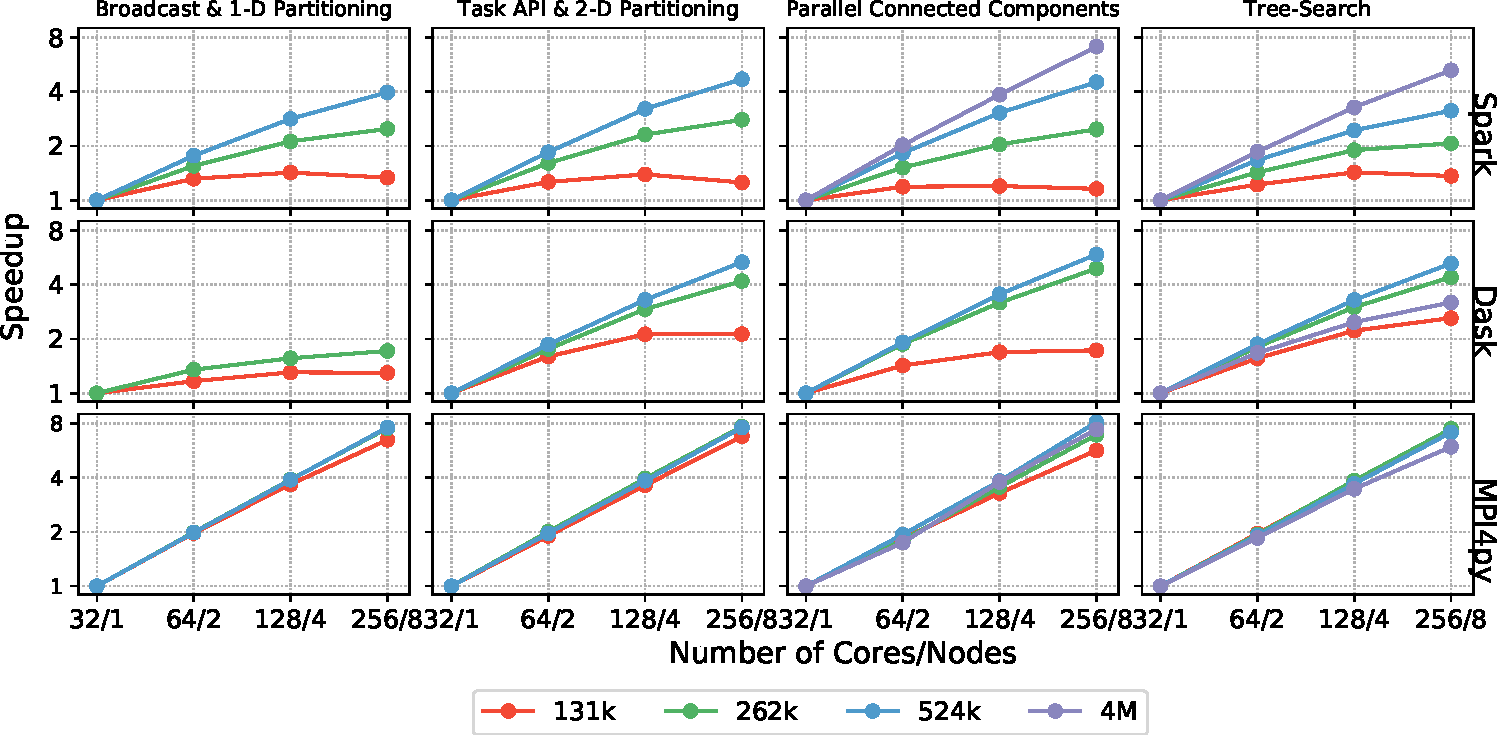
\includegraphics[width=.95\textwidth]{figures/All4approachesWith4MSpeedup.pdf}
    \caption{Selected molecular dynamics analysis MapReduce algorithm speedup for different frameworks and implementation candidates}\label{fig:leafletfinder}
\end{figure*}

The performance analysis of these algorithms implemented in all three 
frameworks provided us with information to create a conceptual model for selecting 
the better suitable framework based on algorithmic characteristics. As shown in Figure~\ref{fig:leafletfinder}, there are cases where the performance of a parallel implementation is far from ideal, while under different circumstances is as expected. Furthermore, non-ideal performance indicates that resource utilization is low. For example in Figure~\ref{fig:leafletfinder}, we see that, based on data sizem Dask provides better speedup than Spark. In these cases Dask better utilized the resources compared to Dask, while on others Spark was better.

Implementation  aspects, such as computational complexity, and shuffled data size influence 
the performance greatly. For embarrassingly parallel applications with coarse grained 
tasks the choice of the framework does not significantly influence performance. 
For fine-grained data parallelism, a data-parallel framework is more suited compared 
to a workload execution framework. In addition, the data shuffling size significantly 
impacts performance and needs to be included in a decision.

Data analysis during scientific campaigns may vary depending on the stage of the 
campaign. As a result, the ability to select the best suited framework, given 
requirements and constraints to execute it is important. This work allows us to 
create that decision making process and include it in the proposed work.

\subsection{Data Analysis Design Selection}

\gpnote{Write about publication number 2}

\section{Proposed Research}

In our research so far, we discussed a conceptual model for data analytics for 
various use cases on HPC system, and a design comparison and execution time model 
for scientific workflows. In addition, we identified a need for execution of 
scientific workflows with minimum user intervention, independent from users' 
scientific domain. In this section, we motivate and propose an autonomic middleware 
for configuring, monitor and adapting the execution of scientific workflows on 
HPCs.

\subsection{Proposed Topic}

Scientific application workflows properties, such as size, and requirements, such as type and number of resources, change in time. In scientific campaignThese properties of the workflow are not necessarily captured during the specification of the workload. 

bla bla workload manager autonomic IBM~\cite{ibm2005autonomic}

Monitoring, regulating, and configuring large scale scientific workflows require 
dedicated human resources that may not be available at any given point in time. 
Autonomic systems offer self-monitoring, self-configuring, and self-regulating 
capabilities. These capabilities can enable execute a scientific 
workflow on HPC resources without user intervention. Incoorporated in a workflow management system a user can define a workflow, desired resources and expeted time to 
completion. The workflow system will then be responsible 
to select how these resources will be used to execute the workflow in terms of concurrency, 
resource type (CPU, GPU) and walltime.

We propose creating an autonomic middleware that will be able to offer these 
\textit{self-*} properties to scientific workflows. This middleware will be 
responsible in monitoring, configuring and regulating the execution based on 
policies and rules defined by the users. 

Self-configuration is achieved by the software deciding the number of resources 
an execution will use to achieve a specific deadline. The middleware will take as 
input models for execution time, memory utilization, storage requirements of kernels used in the workflow. The distribution of the input dataset can also be provided. Based on models 
and a user's deadline it will make a decision how to configure the requested 
resources. That decision includes, but not limited to, number of cores, GPUs, 
type of memory size, and walltime.

Self-monitoring is achieved via the middleware being able to monitor and sample 
the execution state of the workflow. A state full workflow execution engine, such as 
RADICAL-Enseble Toolkit~\cite{balasubramanian2018harnessing}, or Dask~\cite{rocklin2015dask}, 
is required. Such an engine allows the middleware to know the state of the workflow 
at any given point in time. This information can then be used to evaluate the 
configuration decision made.

Self-regulation is achieved by updating the decision during runtime to reflect 
knowledge obtained via monitoring. In addition, the decision making process 
is also updated. Based on the sampled state of execution, and the probability 
of achieving the defined goal, the system will adjust the execution of the 
workflow. If the initial decision was an underestimation, 
more resources can be added. When the decision was an overestimation, the heuristic 
can be updated such that less resources are used in a subsequent execution.

A conceptual architecture is provided by Jha et al. in Ref.~\cite{jha2009self}. 
This architecture consists of a resource manager, an autonomic tuner and an application. 
It defines an Application objective, which is then translated to a set of measurable 
requirements, using well defined metrics, that the application should meet. These 
objectives are achieved through user defined mechanisms. Based on the objective and 
a set of mechanisms, the system can then define necessary strategies and actions to 
achieve the objective.

RADICAL-Ensemble Toolkit~\cite{balasubramanian2018harnessing} (EnTK) defines 
an application manager (AM), and a resource manager (RM). EnTK defines an 
application as a sequence of workflows that are executed. The workflows may 
either reuse resources or request new ones, based on how the user has programmed 
the application. In addition, the time requested for each resource is also 
decided by the user. The AM currently submits a workflow to the resources 
managed by RM and checks their overall execution state. In addition, the resource 
manager requests computing resource from an HPC and monitors their state. None 
of these components have any decision capabilities.

\begin{figure*}[t]
    \centering
    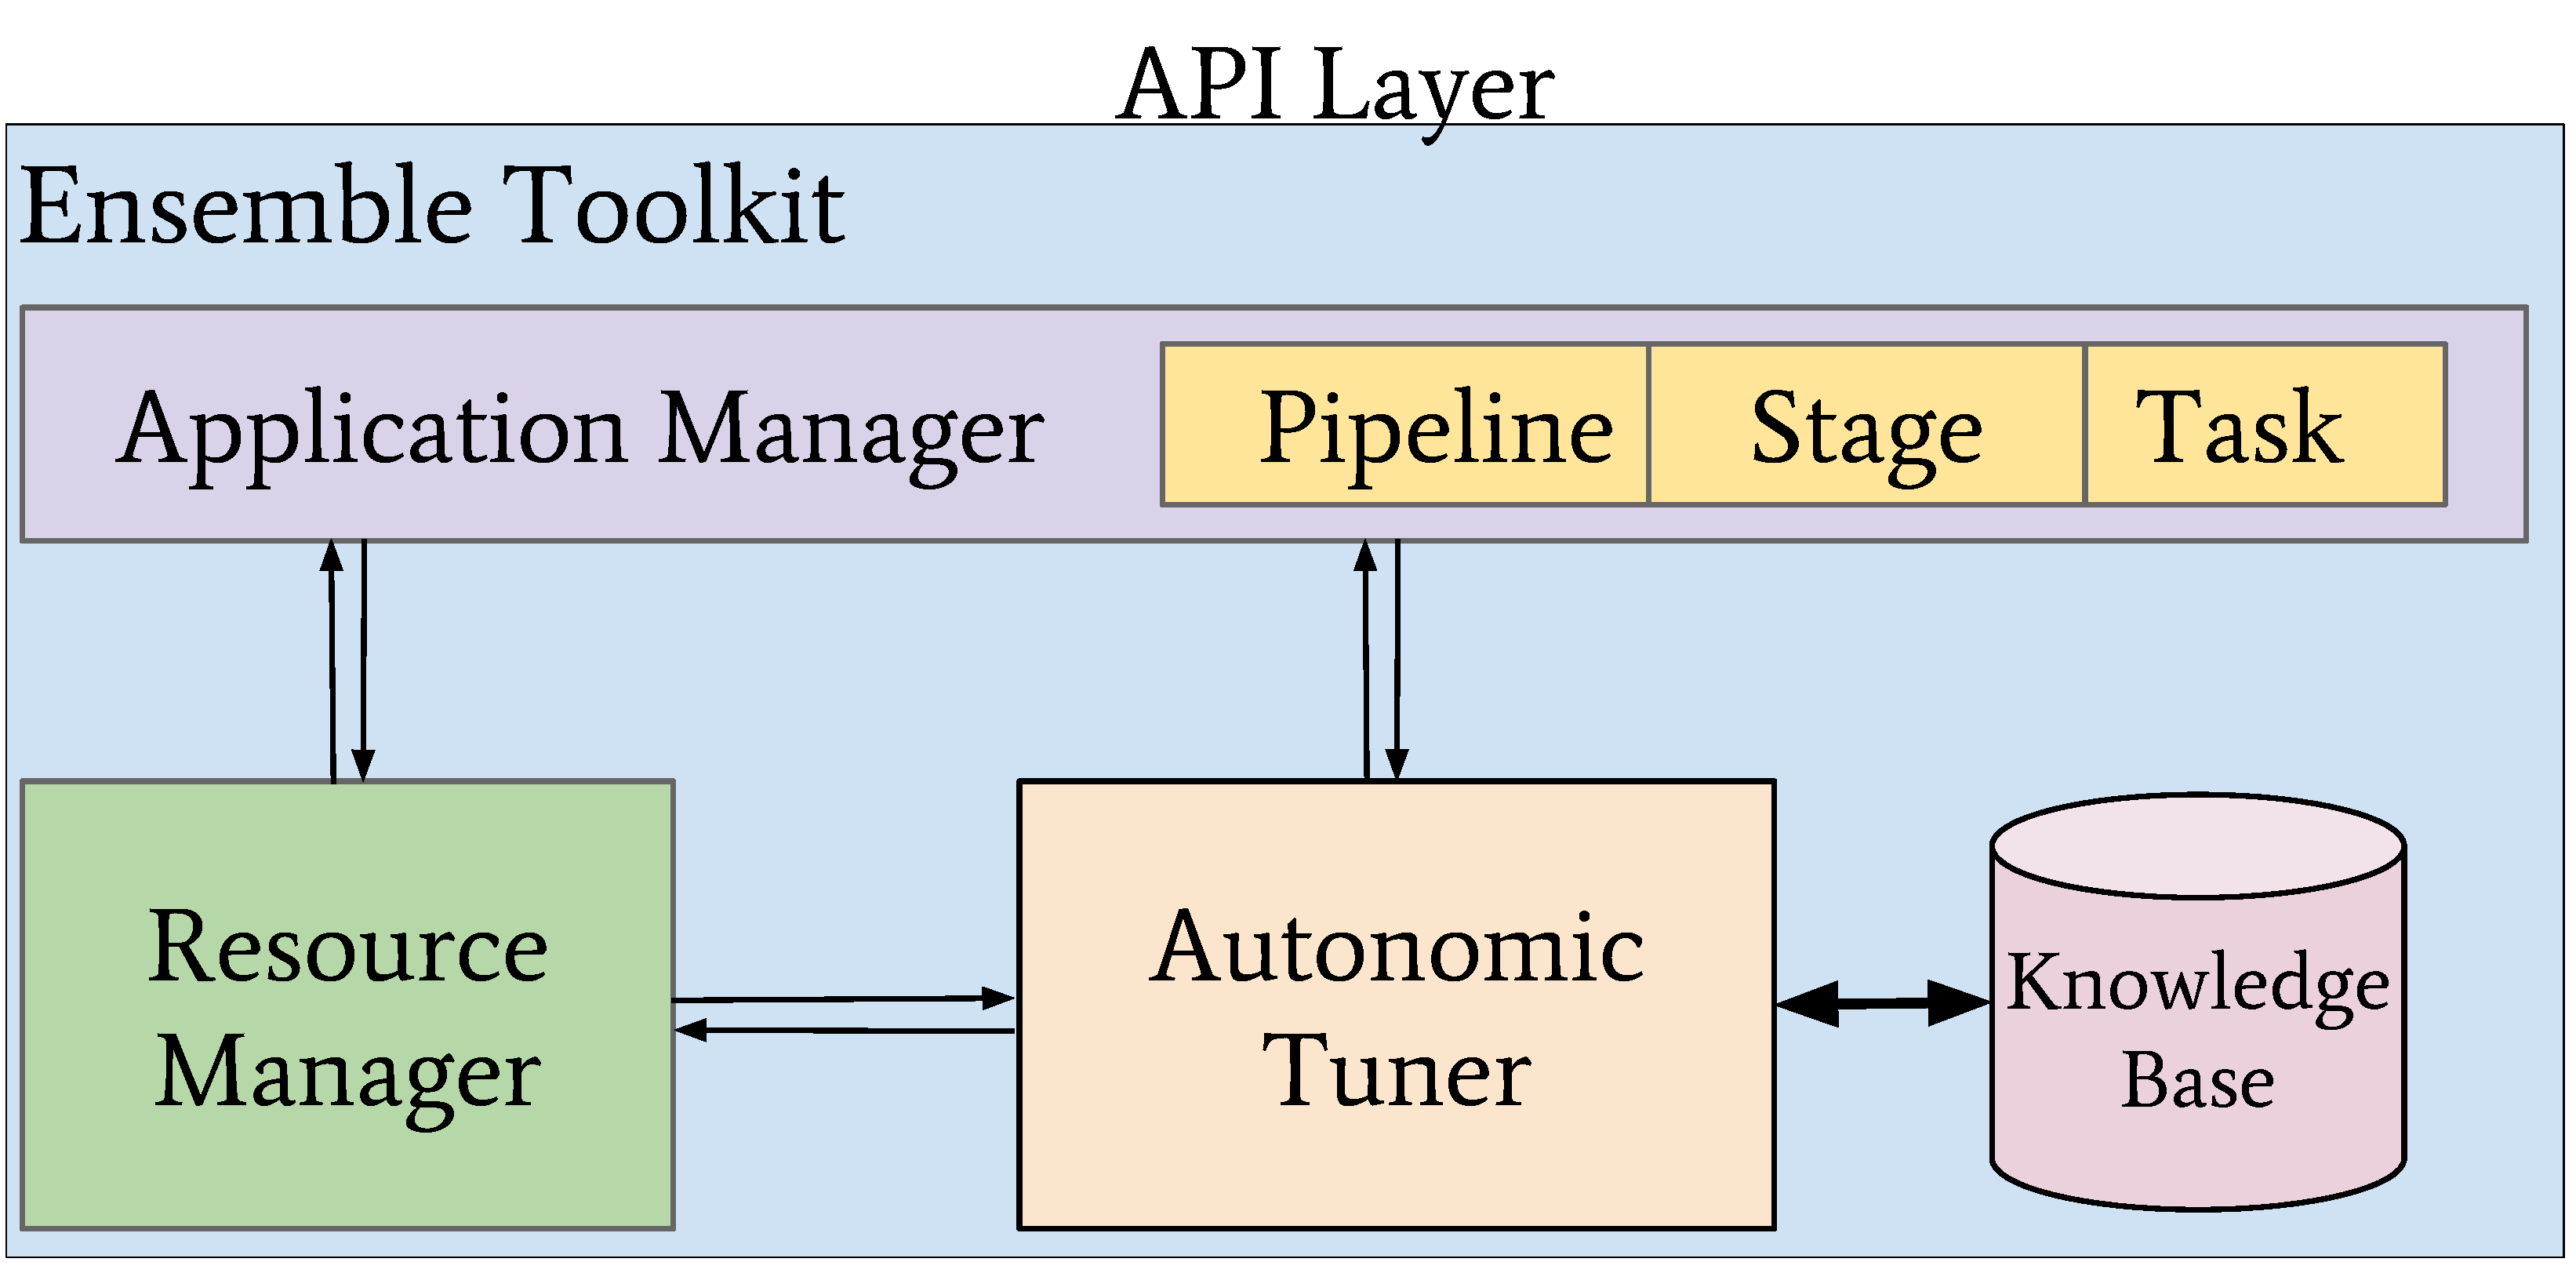
\includegraphics[width=.95\textwidth]{figures/AutonomicSubsystem.pdf}
    \caption{Simple Architectural Diagram. The Application Manager through 
        EnTK's API receives a workflow, a resource request, and a deadline and 
        communicates to the Autonomic Tuner. Autonomic Tuner, based on information 
        in Knowledge Base makes a decision and passes it to the Resource Manager.
        Based on information of the execution state of the workflow the Autonomic
        Tuner updates the knowledge base and its decision}\label{fig:architecture}
\end{figure*}

We propose to extend these two components of EnTK and introduce an autonomic 
tuner, as defined in Ref~\cite{jha2009self}. The AM, apart from the workflow 
definitions, can take as input information of the desired resources to execute 
the workflow, and an Application objective. Initially, the application objective
could be as simple as an execution deadline, but it should be easily extansible to other
metrics. The resource manager based 
on the desired resources can provide information about them, such maximum allowed 
node requests, maximum queue times, and more. The autonomic tuner, we propose 
to add, can use this information along with execution models for the workflow 
tasks to decide concurrency and timeline of the execution of 
the application. This achieves the self-configuration property of an autonomic 
system. The AM already monitors the execution state and it can report it to the 
tuner in specified intervals, achieving this way the self-monitoring property. 
The tuner then can decide whether more resources are required for achieving the 
deadline and update the decision rule, thus achieving the self-regulating aspect 
of an autonomic system. The resource manager acquires and monitors resource 
availability as they are needed by the tuner's decisions. In addition, the resource manager
will provide information about which resources a workflow is executing.
Figure~\ref{fig:architecture} shows a simple diagram of the 
architecture of the proposed extension. The Knowledge Base holds information such as 
execution models of the workflow, and historic data from previous executions.

Changing the number of resources used executing a workflow in HPC resources is not
trivial. When more resources are required to a achieve a deadline, the workflow system
through its autonomic capabilities can request as many computational nodes as needed. 
On the other hand, when resources are underutilized, the autonomic system should either
release part of them or update the decision for subsequent runs. Nodes on HPCs can be
requested either as single or multiple nodes. Since many resources have policies at place
to regulate the total number of concurrent jobs a user has, it is preferable to request
nodes in numbers larger than one. That requires, whenever resources are released, to
release them also as multiple nodes. Initially, we will assume that our workflows do not
underutilize the resources.
\gpnote{Talk about EnTK's AppManager. See how an autonomic system controller can
be added to extend it. It makes sense that each app manager will be able to 
decide it self about the execution of a workflow. }


\subsection{Proposed Timelime}
\begin{figure*}[t]
	\centering
	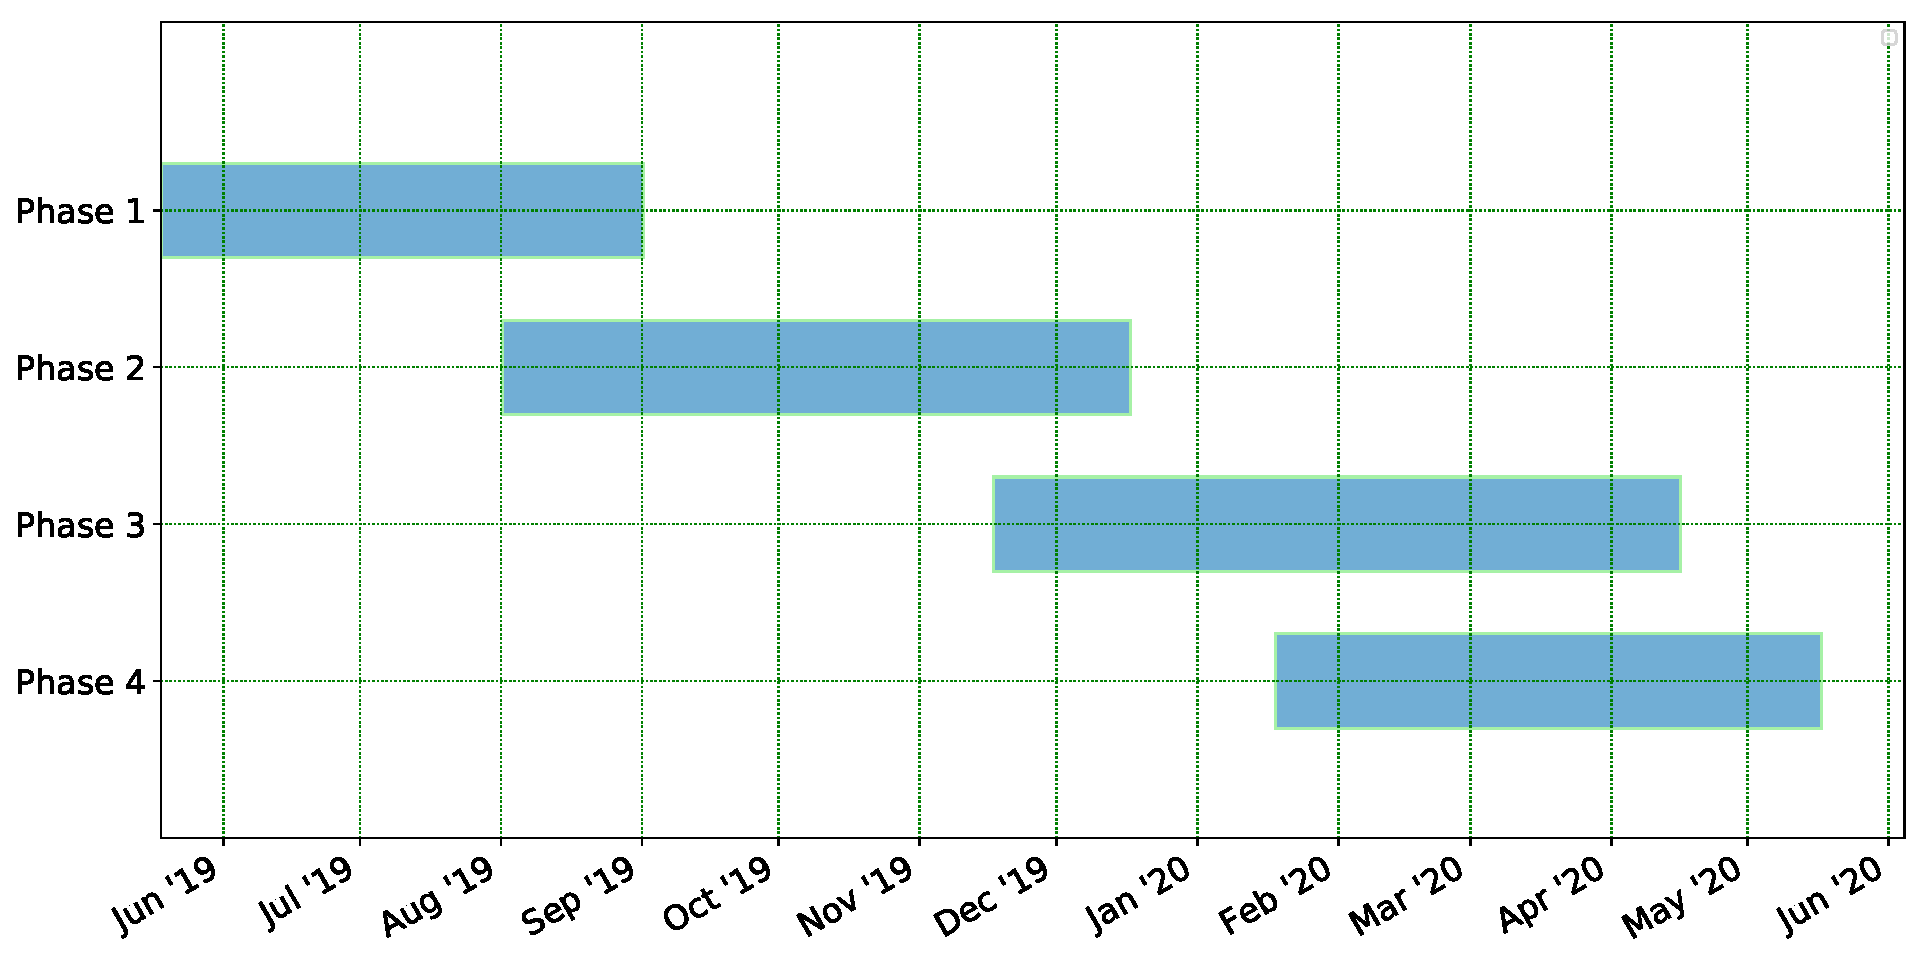
\includegraphics[width=.95\textwidth]{figures/phd_plan.pdf}
	\caption{Planned timeline of proposed research}\label{fig:work_plan}
\end{figure*}

\subsubsection{Phase 1: Design and implementation self-configuring property}

Month 1 would include design discussions for a prototype of the execution system. 
Result of these discussions will be the requirements of the middleware and its 
API. Design will be finalized and a prototypical implementation will be completed 
by Month 4. Capability to self-configure in terms of resources based on the desired 
workflow will mark the success of Phase 1.

\subsubsection{Phase 2: Implementation self-monitoring, self-regulating properties
and Continuous Integrated Testing}
Phase 2 includes defining the requirements for self-monitoring, and self-regulating 
properties and implement them in the middleware. End of phase 2 will include the 
\textit(self-*) properties as well as a Continuous integrated testing protocol to 
always verify the functionality of the middleware. Phase 2 spans from months 3 up 
to 6

\subsubsection{Phase 3: Integration with scientific workflows}
Phase 3 of the plan includes the integration of the proposed autonomic system with 
RADICAL-EnTK~\cite{balasubramanian2018harnessing} and start utilize the system for 
scientifc workflows in Satelite Imagery analysis and Molecular Dynamics simulation 
workflows. This phase spans between months 6 and 9.

\subsubsection{Phase 4: Investigation for an empirical model}

Experiments with synthetic and real applications with the prototype as well as 
scientific workflows will be used to investigate and derive empirical models. 
These models may be used to further generalize the behavior of the autonomic 
middleware based on application requirements. Phase 4 will overlap with Phase 2 
and 3 to utilize experiments done during those phases.

% ---------------------------------------------------------------------------
% Why
\subsection{Significance and impact of work}
Several scientific applications are required to be executed several times with 
different input data or initial conditions. The required concurrency to minimize 
the execution time of each run is not necessarily constant and may change based 
on the initial conditions. The autonomic management system suggested in this 
proposal will be the first to make resource configuration decisions for the users. 
This will lead to less time invested by users to make execution decisions about 
their workflows. These decisions will lead to better resource utilization and, 
as a result, better domain science. The empirical models derived by this work can 
be used to derive formal mathematical models.

% ---------------------------------------------------------------------------
% Challenges
\subsection{Challenges/Risks}

We estimate the proposed work, divided into four major phases, to take 12 months 
and we allocate 3 months to account for unforeseen circumstances. We would like 
to keep the committee aware of the following challenges that we see:

\begin{itemize}
	\item Design and Implementation (phases 1 \& 2) is iterative and special attention 
	needs to be given to the number of iterations against specific objectives, 
	given the timeline.
  \item All experiments performed on HPC systems are subject to variable queue 
	times and may limit the number of experiments performed in phase 2 and 4.
	\item Although the middleware will be well tested (80--90\% of the code base 
	will be covered by unit tests) and less susceptible to major changes, RADICAL-Pilot 
	is known to be less stable and is susceptible to changes as it serves multiple 
	projects. Stability of RADICAL-Pilot is considered in the estimates, but needs 
	to be made aware to the committee.
	\item Lastly, the HPC systems themselves may often become inaccessible due to 
	unplanned outages.
\end{itemize}

\bibliographystyle{plain}
\bibliography{proposal}
\end{document}\textit{}